% Copyright (C) 2012 Shi.Zhan <g.shizhan.g@gmail.com>
%
% Permission is hereby granted, free of charge, to any person obtaining a copy of this software and associated documentation files (the "Software"), to deal in the Software without restriction, including without limitation the rights to use, copy, modify, merge, publish, distribute, sublicense, and/or sell copies of the Software, and to permit persons to whom the Software is furnished to do so, subject to the following conditions:
%
% The above copyright notice and this permission notice shall be included in all copies or substantial portions of the Software.
%
% THE SOFTWARE IS PROVIDED "AS IS", WITHOUT WARRANTY OF ANY KIND, EXPRESS OR IMPLIED, INCLUDING BUT NOT LIMITED TO THE WARRANTIES OF MERCHANTABILITY, FITNESS FOR A PARTICULAR PURPOSE AND NONINFRINGEMENT. IN NO EVENT SHALL THE AUTHORS OR COPYRIGHT HOLDERS BE LIABLE FOR ANY CLAIM, DAMAGES OR OTHER LIABILITY, WHETHER IN AN ACTION OF CONTRACT, TORT OR OTHERWISE, ARISING FROM, OUT OF OR IN CONNECTION WITH THE SOFTWARE OR THE USE OR OTHER DEALINGS IN THE SOFTWARE.
%
% 课程:人机交互技术及应用
% 班级:传播学1001班
% 课时:40学时,2012年秋季1~10周,每周一、三
% 地点:东九楼D212
% 主页:http://code.google.com/p/hci-course/
% 教师:施展 
% 单位:华中科技大学 武汉光电国家实验室
%
\documentclass{beamer}
\usepackage{fontspec,xunicode,xltxtra,beamerthemesplit}
%\usetheme{Hannover} % White background
\usetheme{Berkeley} % Blue background
\setsansfont[Mapping=tex-text, ItalicFont={Courier Italic}]{Microsoft YaHei}

% 中文环境自动换行
\XeTeXlinebreaklocale "zh"
\XeTeXlinebreakskip = 0pt plus 1pt

% 中文环境修正导航栏
\makeatletter
\def\beamer@linkspace#1{
	\begin{pgfpicture}{0pt}{-1.5pt}{#1}{5.5pt}
		\pgfsetfillopacity{0}
		\pgftext[x=0pt,y=-1.5pt]{.}
		\pgftext[x=#1,y=5.5pt]{.}
	\end{pgfpicture}
}
\makeatother

% diagrams
\usepackage{tikz}
\usetikzlibrary{trees,arrows,chains,shapes}

% full page image
\newcommand{\fullPageImage}[2]{
	{
		\usebackgroundtemplate{\includegraphics[width=\paperwidth, height=\paperheight]{#1}}
		\frame[plain]{#2}
	}
}

\title{人机交互技术}
\author{施展}
\institute{华中科技大学~武汉光电国家实验室}
\date{\today}
\titlegraphic{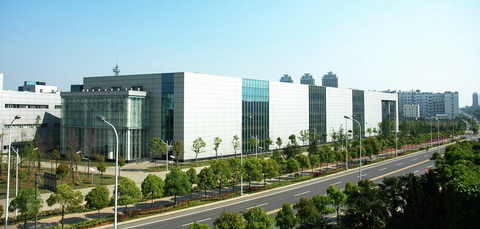
\includegraphics[width=2cm]{images/wnlo.jpg}}

\begin{document}

\begin{frame}
	\titlepage
\end{frame}

\begin{frame}
	\frametitle{内容提要}
	\tableofcontents
\end{frame}

\section{第三讲}
\begin{frame}
	\frametitle{第三讲 交互设备}
	\begin{itemize}
%		\item 了解文本输入设备,图像输入设备,指点输入设备,掌握三维图形输入设备
		\item 了解文本输入设备,图像输入设备,触摸屏输入设备,体感输入设备
%		\item 了解显示器,声音的输出,数字纸等输出设备
		\item 了解显示器,声音的输出,电子墨水等输出设备
%		\item 了解虚拟现实交互设备
	\end{itemize}
\end{frame}

\subsection{输入设备}
\begin{frame}
	\frametitle{输入设备}
	\begin{center}
	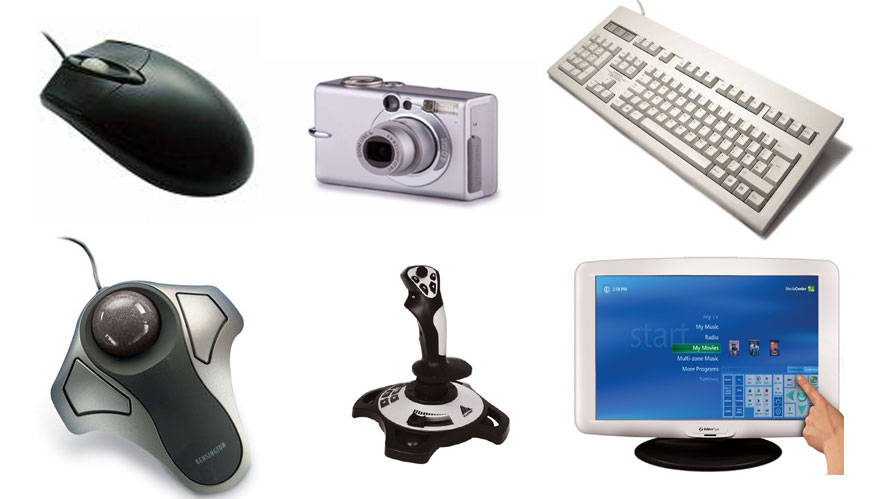
\includegraphics[width=\textwidth]{images/input-devices.jpg}
	\end{center}
\end{frame}

\subsubsection{文本输入设备}
\begin{frame}
	\frametitle{文本输入设备}
	\begin{itemize}
		\item 文本输入是人与计算机交互的一个重要组成部分,同时也是一项繁重的工作。
		\begin{itemize}
			\item 键盘为主
			\item 手写、识别(字符/条码、图像、语音)为辅
		\end{itemize}
	\end{itemize}
\end{frame}

\begin{frame}
	\label{lecture03:keyboard}
	\frametitle{键盘 Keyboard}
	\transglitter % Glitter sweeps in specified direction
	\transduration<1,2,3>{.2} % Show slide specified number of seconds

	% preparation
	\tikzstyle{imagenode} = [anchor=north west]
	% Usage:
	% \tikzoverlay at (-1cm,-5cm) {content};
	% or
	% \tikzoverlay[text width=5cm] at (-1cm,-5cm) {content};
	\def\tikzoverlay{%
		\tikz[baseline,overlay]\node[imagenode]
	}%

	\tikzoverlay at (0cm,-3cm) {文本输入最主要手段~{\tiny 应用环境影响布局,布局影响速度、准确性、舒适度。}};\pause
	\tikzoverlay at (3cm, 4.5cm) {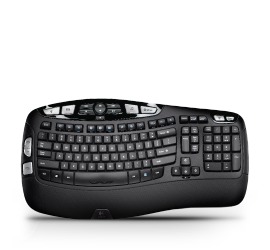
\includegraphics[width=5cm]{images/keyboard.png}};\pause
	\tikzoverlay at (0cm, 0cm) {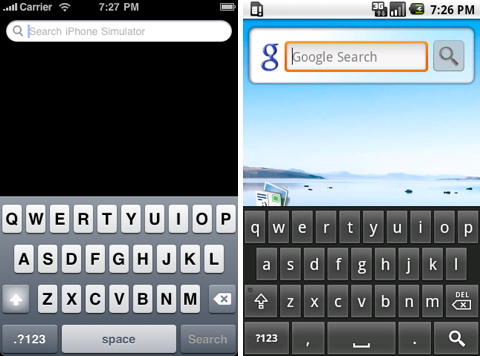
\includegraphics[width=3cm]{images/mobile_keyboards.png}};\pause
	\tikzoverlay at (6cm, 0cm) {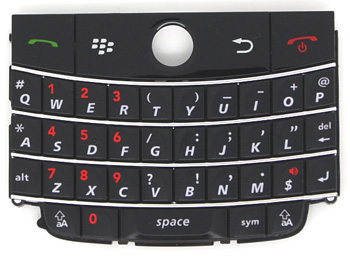
\includegraphics[width=3cm]{images/blackberry-bold-9000-keyboard.jpg}};
\end{frame}

\begin{frame}
	\frametitle{键盘分类}
	\beamertemplatetransparentcovereddynamicmedium
	\begin{itemize}
		\item 编码键盘
		\begin{itemize}
			\item 控制电路的功能完全依靠硬件自动完成,能自动将所按下的按键的编码信息送入计算机。
			\item 响应速度快,但硬件结构复杂。
		\end{itemize}\pause
		\item 非编码键盘
		\begin{itemize}
			\item 控制电路功能要依靠硬件和软件共同完成。
			\item 虽然响应速度不如编码键盘快,但可通过软件为键盘的某些按键重新定义,容易扩充键盘功能,应用广泛。
		\end{itemize}
	\end{itemize}
\end{frame}

\begin{frame}
	\frametitle{键盘布局}
	\begin{itemize}
		\item QWERTY键盘布局
		\begin{itemize}
			\item 19世纪70年代,Christopher Sholes发明了QWERTY键盘布局,其名称来源于该布局方式最上行前6个英文字母,最常用的几个字母安置在相反方向,最大限度放慢敲键速度以避免卡键。
			\item 这种布局方式依然是今天最为常见的排列方式{\tiny (第\ref{lecture03:keyboard}页)},成为一种事实上的标准。
		\end{itemize}
	\end{itemize}
	\begin{center}
	% http://zh.wikipedia.org/wiki/QWERTY鍵盤
	% http://upload.wikimedia.org/wikipedia/commons/3/3a/Qwerty.svg
	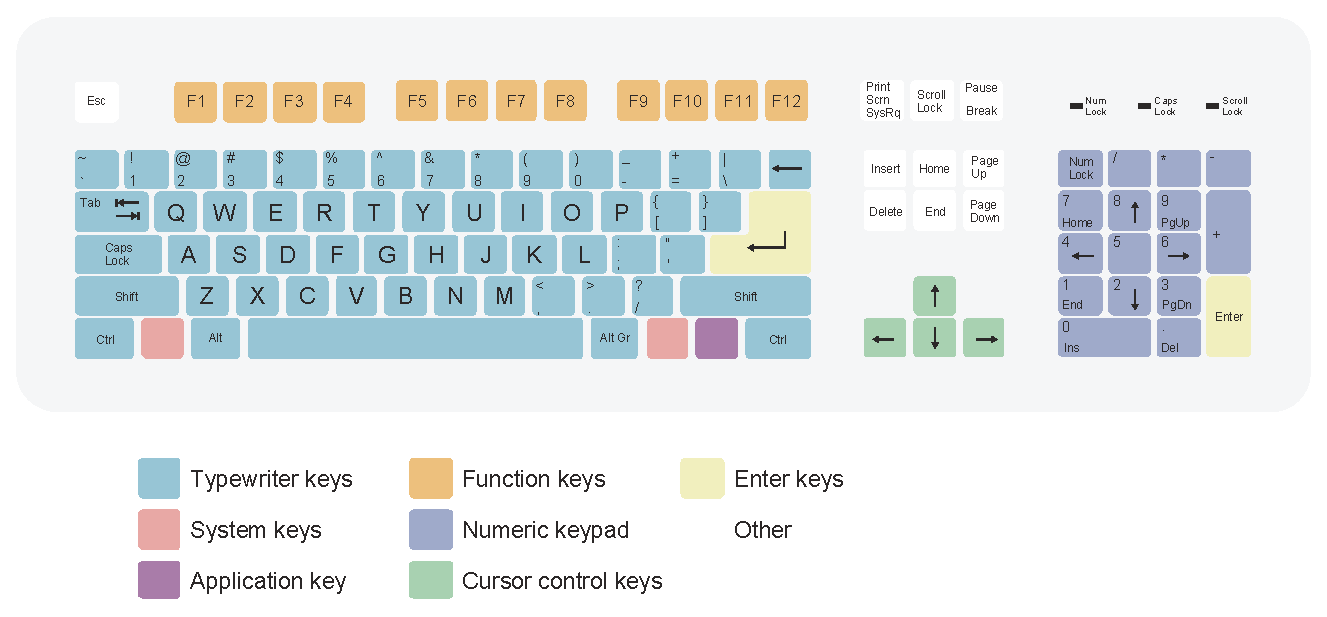
\includegraphics[width=8cm]{images/qwerty.eps}
	\end{center}
\end{frame}

\begin{frame}
	\frametitle{键盘布局}
	\begin{itemize}
		\item DVORAK键盘布局
		% http://www.cnbeta.com/articles/120272.htm
		% http://baike.baidu.com/view/1410112.htm
		\begin{itemize}
			\item 20世纪20年代的DVORAK键盘布局,据推测使用DVORAK,打字者的手指平均每日运动1英里,而QWERTY则是12到20英里。
			\item DVORAK可以大大减少手指移动距离,从而大大提高输入速度,但由于受到传统QWERTY布局的影响,没有成为主流的键盘布局。
		\end{itemize}
	\end{itemize}
	\begin{center}
	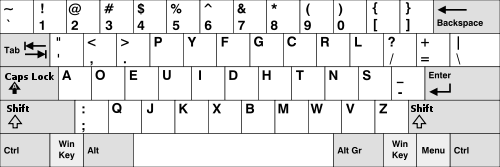
\includegraphics[width=8cm]{images/dvorak.png}
	\end{center}
\end{frame}

\begin{frame}
	\frametitle{人机工程学键盘 Ergonomic Keyboard}
	%\beamertemplatetransparentcovereddynamicmedium
	\transdissolve
	% the above can't be used since it will prevent the picture to show correctly
	% http://www.hudong.com/wiki/人体工学键盘
	% http://www.osha.gov/SLTC/etools/computerworkstations/components_keyboards.html
	% http://www.ergonomics-info.com/computer-ergonomic-keyboard.html
	\begin{center}
		\onslide<1->{
			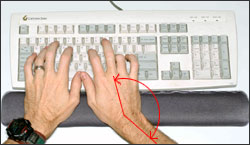
\includegraphics[width=3cm]{images/comp_keyboard_angledwrist.jpg}~
			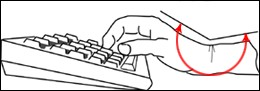
\includegraphics[width=4cm]{images/comp_keyboard_bent_wrist.jpg}\\
			{\tiny 长时间悬腕或塌腕将造成关节劳累——腕管综合征}\\
		}
		\onslide<2->{
			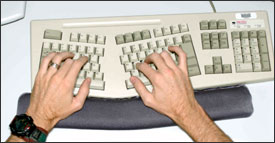
\includegraphics[width=3cm]{images/comp_keyboard_ergo.jpg}~
			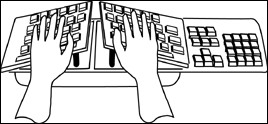
\includegraphics[width=4cm]{images/comp_keyboard_tented.jpg}\\
			{\tiny 将两手所控的键位向两旁分开一定的角度,使两臂自然分开,缓解臂、腕疲劳}\\
		}
		\onslide<3->{
			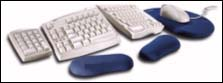
\includegraphics[width=4cm]{images/alternative_keyboard.jpg}~
			{\tiny 增加腕托}
		}
	\end{center}
\end{frame}

\begin{frame}
	\frametitle{人机工程学键盘 Ergonomic Keyboard}
	\transdissolve
	\begin{itemize}
		\onslide<1->{\item 目前这类键盘品种很多,有固定式、分体式和可调角度式,以适应不同操作者的各种姿势。}
		\onslide<2->{
			\item {\tiny 微软自然键盘 Microsoft Nature Keyboard}\\
			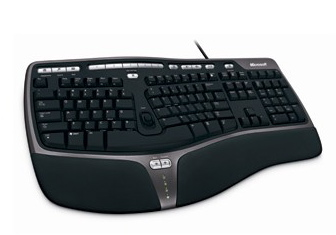
\includegraphics[width=3.5cm]{images/microsoft-natural-ergonomic-keyboard-4000.jpg}~
			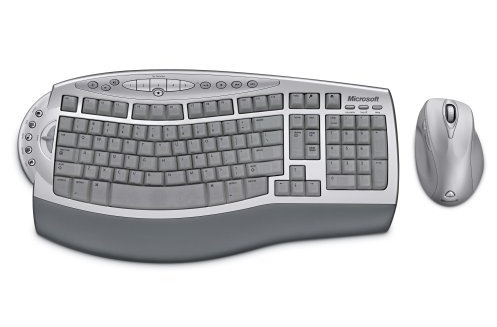
\includegraphics[width=3.5cm]{images/ergonomic-keyboard-mac-microsoft.jpg}
		}
		\onslide<3->{
			\item {\tiny \textbf{Kinesis}, \textbf{Logitech} 人体工学键盘 \dots}\\
			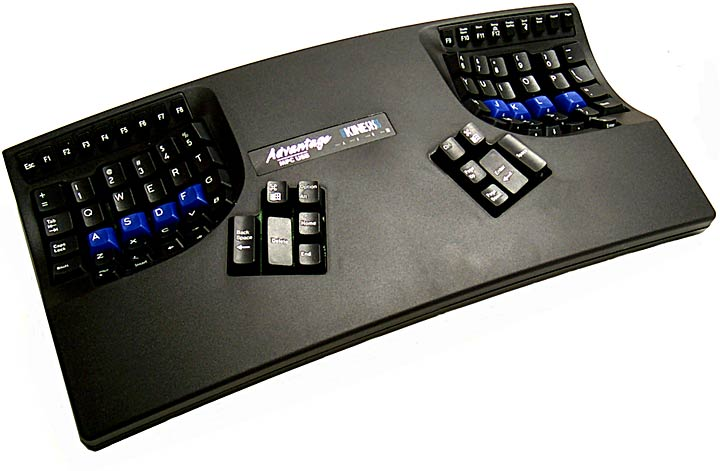
\includegraphics[width=3.5cm]{images/kinesis-advantage-keyboard.jpg}~
			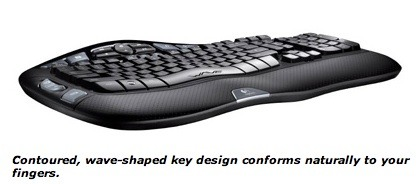
\includegraphics[width=3.5cm]{images/logitech-ergonomic-keyboard-wave.jpg}
		}
	\end{itemize}
\end{frame}

\begin{frame}[transdissolve]
	\frametitle{人机工程学键盘 Ergonomic Keyboard}
	\begin{itemize}
		\item 分体式人体工学键盘 Modular Ergonomic Keyboard\\
		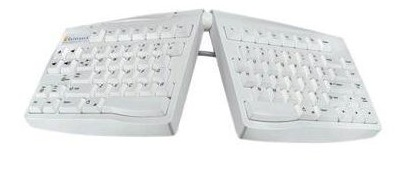
\includegraphics[width=4cm]{images/ergonomic-keyboard-mac-goldtouch.jpg}~
		% http://elecinlife.com/modular-ergonomic-keyboard-falls-to-pieces/
		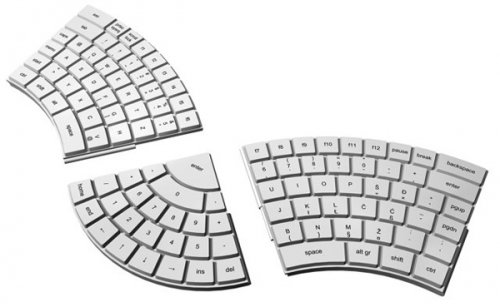
\includegraphics[width=4cm]{images/ergonomic-modular-keyboard-falls-to-pieces_1.jpg}\\
		\begin{center}
		% http://c2.com/cgi/wiki?KinesisEvolutionKeyboard
		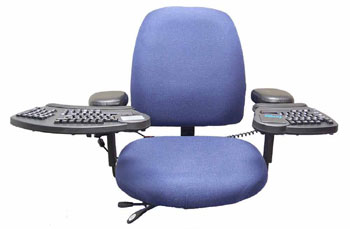
\includegraphics[width=4cm]{images/keyboard-chair.jpg}
		\end{center}
	\end{itemize}
\end{frame}

\begin{frame}
	\frametitle{多功能集成键盘}
	\transdissolve
	\begin{itemize}
		\item 游戏、无线、DJ\\
		% http://www.coolest-gadgets.com/20071120/hybrid-gaming-keyboard-gives-you-all-the-keys-you-need-but-you-still-cant-type-well-on-it/
		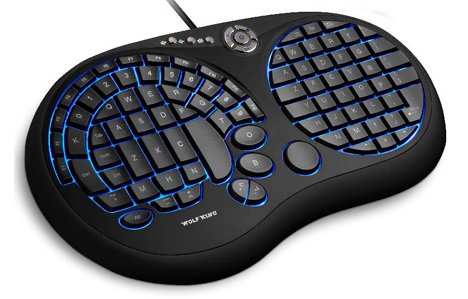
\includegraphics[width=4cm]{images/wolfking-warrior-xxtreme.jpg}~
		% http://achknowledge.wordpress.com/2011/06/23/best-gaming-keyboard-and-mouse/
		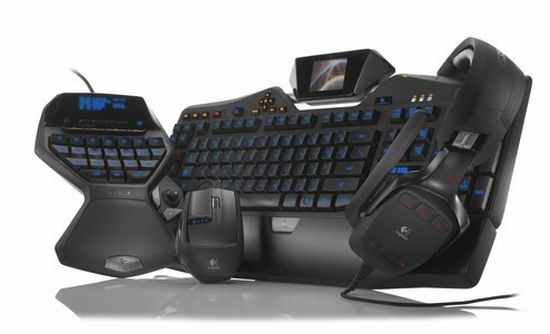
\includegraphics[width=4cm]{images/logitech-g19-gaming-keyboard.jpg}\\
		% http://www.walmart.com/ip/The-Singing-Machine-Sound-X-Kids-Electronic-Keyboard-DJ-Mixer/17133266
		\begin{center}
		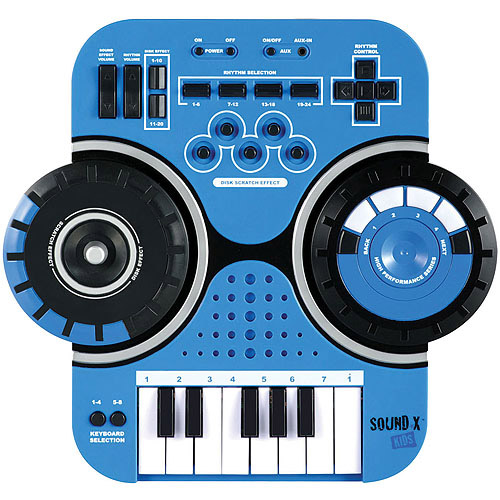
\includegraphics[width=3cm]{images/sound-x-electronic-keyboard-dj-mixer.jpg}
		\end{center}
	\end{itemize}
\end{frame}

\begin{frame}
	\frametitle{手写设备}
	\begin{itemize}
		\item 手写板+手写笔\\
		{\tiny 除用于文字、符号、图形等输入外,还可提供光标定位功能,从而同时替代键盘与鼠标}
	\end{itemize}
	% http://m.pconline.com.cn/shop123090/nid:3118168/news_detail.html
	\begin{center}
		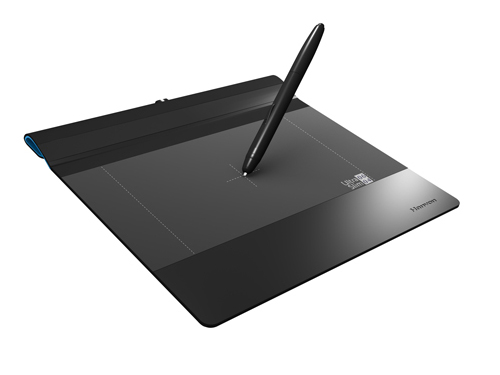
\includegraphics[width=4cm]{images/drawing-pad-hanwang.jpg}~
		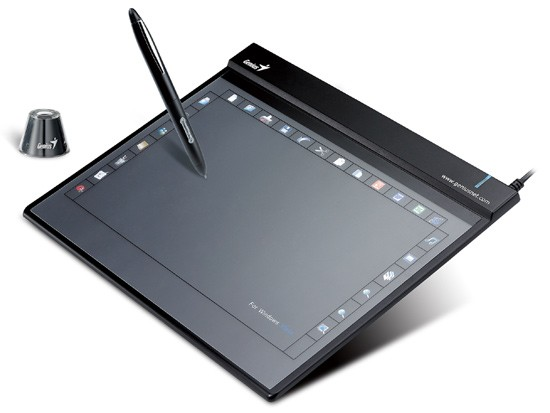
\includegraphics[width=4cm]{images/drawing-pad-mengtian.jpg}
	\end{center}
\end{frame}

\begin{frame}
	\frametitle{手写板}
	% http://baike.baidu.com/view/207382.htm
	\begin{itemize}
		\item 电阻式压力手写板:\\{\tiny 几乎已经被淘汰}
		\item 电磁式感应手写板:\\{\tiny 目前市场主流产品}
		\item 电容式触控手写板:\\{\tiny 市场的新生力量,具有耐磨损、使用简便、敏感度高等优点,是今后手写板的发展趋势。}
	\end{itemize}
\end{frame}

\begin{frame}
	\frametitle{光学字符识别 Optical Character Recognition}
	\beamertemplatetransparentcovereddynamicmedium
	% http://baike.baidu.com/view/17761.htm
	\begin{itemize}[<+->]
		\item 对文本资料的图像文件进行分析处理,获取文字及版面信息的过程。
		\item 在1929年由德国科学家Tausheck最先提出来的,后来美国科学家Handel也提出了利用技术对文字进行识别的想法。
		\item 最早对印刷体汉字识别进行研究的是IBM公司的Casey和Nagy,1966年他们发表了第一篇关于汉字识别的文章,采用了模板匹配法识别了1000个印刷体汉字。
		\item 20世纪70年代初,日本的学者开始研究汉字识别,并做了大量的工作。
		\item 中国在OCR技术方面的研究工作起步较晚,70年代末开始进行汉字识别的研究,80年代产品化。
	\end{itemize}
\end{frame}

\begin{frame}
	\frametitle{光学字符识别 Optical Character Recognition}
	\tikzstyle{treenode}	= [draw=black,thick,anchor=west]
	\tikzstyle{comment}		= [fill=gray!80,anchor=west]
	\begin{tikzpicture}[%
		grow via three points={one child at (0.5,-0.7) and
		two children at (0.5,-0.7) and (0.5,-1.4)},
		edge from parent path={(\tikzparentnode.south) |- (\tikzchildnode.west)}]
		\node [treenode] {光学字符识别}
			child { node [treenode] {图像处理模块}
				child { node [comment] {文稿扫描、图像缩放、图像旋转}}}
			child [missing] {}	
			child { node [treenode] {版面划分模块}
				child { node [comment] {版面划分、更改划分~{\tiny 理解版面、字切分、归一化等}}}}
			child [missing] {}
			child { node [treenode] {文字识别模块}
				child { node [comment] {{\tiny 逐行切割、单字辨认、归一化、特征提取、识别}}}}
			child [missing] {}
			child { node [treenode] {文字编辑模块}
				child { node [comment] {文字修改、编辑}}};
	\end{tikzpicture}
\end{frame}

\begin{frame}
	\frametitle{光学字符识别 Optical Character Recognition}
	\beamertemplatetransparentcovereddynamicmedium
	\tikzstyle{punktchain}	= [
		rectangle, 
		rounded corners, 
		% fill=black!10,
		draw=black, very thick,
		text width=7em, 
		minimum height=1em, 
		text centered, 
		on chain]
	\tikzstyle{normalchain}	= [
		rectangle, 
		rounded corners, 
		% fill=black!10,
		%draw=black, very thick,
		text width=7em, 
		minimum height=1em, 
		text centered, 
		on chain]
	\tikzstyle{line}	= [draw, thick, <-]
	\tikzstyle{every join}	= [->, thick, shorten >=1pt]
%	影像输入、影像前处理、文字特征抽取、比对识别、人工校正、结果输出
	\begin{columns}
	\column{.4\textwidth}
	\begin{tikzpicture}
		[node distance=.3cm, start chain=going below,]
  		\onslide<1>{\node[normalchain, join] (a) {影像输入};}
		\onslide<2>{\node[punktchain, join] (b) {影像前处理};}
		\onslide<3>{\node[punktchain, join] (c) {文字特征抽取};}
		\onslide<4>{\node[punktchain, join] (d) {比对识别};}
		\onslide<5>{\node[punktchain, join] (e) {人工校正};}
		\onslide<6>{\node[normalchain, join] (f) {结果输出};}
	\end{tikzpicture}
	\column{.6\textwidth}
	\begin{itemize}
		\only<1>{\item 使用光学仪器,如影像扫描仪、传真机或任何摄影器材,将影像转入计算机。}
		\only<2>{\item 影像正规化、去除噪声、影像矫正等的影像处理,及图文分析、文字行与字分离的文件前处理。}
		\only<3>{
			\item 用什么特征、怎么抽取?
			\begin{itemize}
				\item 统计的特征,如文字区域内的黑/白点数比;
				\item 结构的特征,如文字影像细线化后,取得字的笔划端点、交叉点之数量及位置。
			\end{itemize}
		}
		\only<4>{
			\item 使用特征数据库来进行比对。
			\begin{itemize}
				\item 根据不同的特征特性,选用不同的数学距离函数;
				\item 辅以神经网络、专家系统;
				\item 字词后处理:相似候选字群,根据上下文选择。
			\end{itemize}
		}
		\only<5>{
			\item 文字影像与识别文字的对照
			\item 屏幕信息摆放的位置
			\item 每一识别文字的候选字、拒认字
			\item 字词后处理后标示出可能有问题的字词
		}
		\only<6>{\item 格式还原、人工排版}
	\end{itemize}
	\end{columns}
\end{frame}

\begin{frame}
	\frametitle{手写识别 Handwriting Recognition}
	\begin{center}
	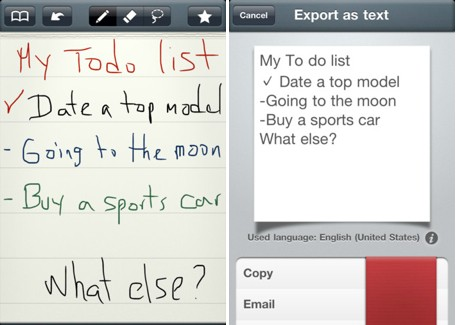
\includegraphics[width=4cm]{images/myscriptmemo7212.jpg}~\pause
	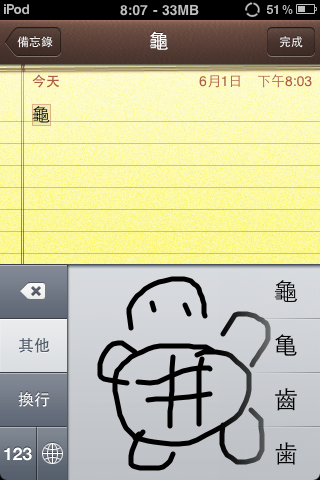
\includegraphics[width=4cm]{images/apple-handwriting.png}
	\end{center}
\end{frame}

\subsubsection{指点输入设备}
\begin{frame}
	\frametitle{指点输入设备}
	\beamertemplatetransparentcovereddynamicmedium
	\transduration<1,2>{.1}
	\begin{itemize}[<+->]
		\item 指点设备常用于完成一些\textbf{定位}和\textbf{选择物体}的交互任务。
		\item 物体可能处于一维、二维、三维或更高维的空间中。
		\item 选择与定位的方式可以是\textbf{直接选择},或通过\textbf{操作屏幕上的光标}来完成。
	\end{itemize}
\end{frame}

\begin{frame}
	\frametitle{鼠标 Mouse}
	\begin{itemize}
	\item 1968年12月9日,世界上的第一个鼠标诞生于美国斯坦福大学,由Douglas Englebart博士发明。
	\end{itemize}
	\begin{center}
	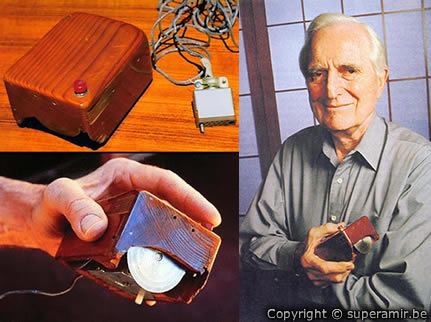
\includegraphics[width=7cm]{images/first-mouse.jpg}
	\end{center}
\end{frame}

\begin{frame}
	\frametitle{鼠标 Mouse}
	\beamertemplatetransparentcovereddynamicmedium
	\begin{columns}
		\column{.6\textwidth}
		\begin{itemize}[<+->]
		\item 外形是一只小木头盒子
		\item 工作原理
		\begin{itemize}
			\item 底部的小球带动枢轴转动,继而带动变阻器改变阻值来产生位移信号,并将信号传至主机。
		\end{itemize}
		\item 鼠标的使用使得计算机的操作更加简便,有效代替了键盘的繁琐指令。
		\end{itemize}
		\column{.4\textwidth}
		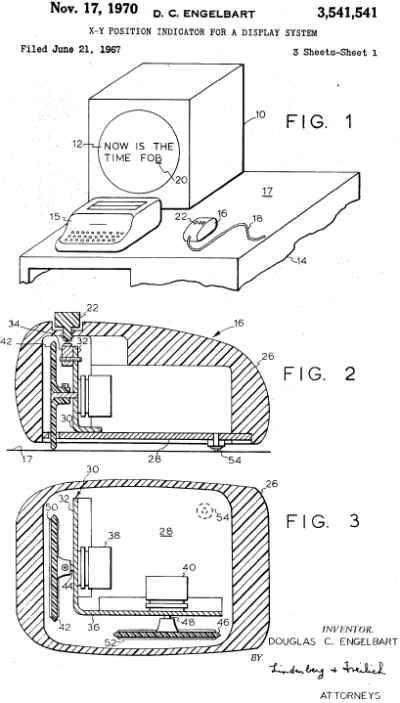
\includegraphics[width=3.5cm]{images/computer-mouse-original-patent.jpg}
	\end{columns}
\end{frame}

\begin{frame}
	\frametitle{鼠标的分类}
	\beamertemplatetransparentcovereddynamicmedium
	\begin{center}
	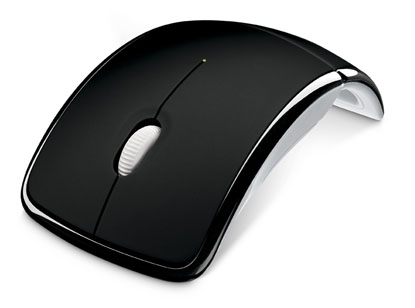
\includegraphics[width=3cm]{images/mouse1.jpg}
	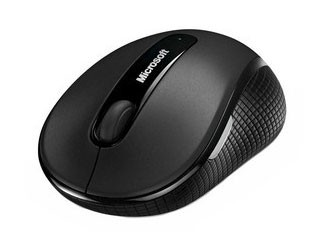
\includegraphics[width=3cm]{images/mouse2.jpg}
	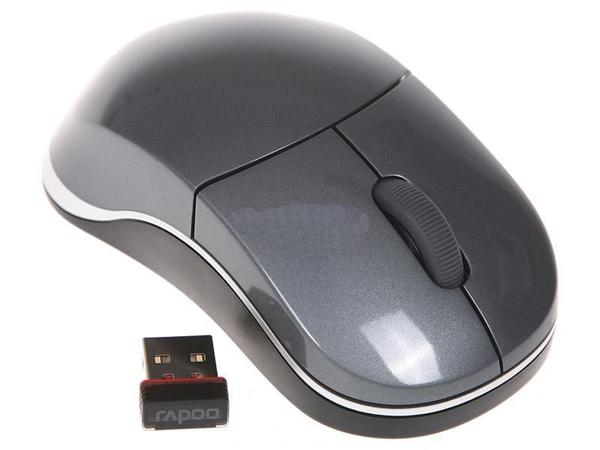
\includegraphics[width=3cm]{images/mouse3.jpg}
	\end{center}
	\begin{itemize}
		\item 依据移动感应技术的分类
		\begin{itemize}
			\onslide<1-6>{\item 机械鼠标}
		    \onslide<2-6>{\item 早期光电鼠标~{\tiny 需要印有特定条纹的鼠标垫}}
		    \onslide<3-6>{\item 光电机械鼠标}
		    \onslide<4->{\item 光电鼠标~{\tiny 现代的“红光鼠标”,无需特定条纹的鼠标垫}}
		    \onslide<5->{\item 蓝光鼠标~{\tiny 民用高端,DPI可达2000}}
		    \onslide<6,7>{\item 激光鼠标~{\tiny DPI高端的能达到5000以上}}
		\end{itemize}
	\end{itemize}
\end{frame}

\begin{frame}
	\frametitle{鼠标与计算机的接口}
	\begin{itemize}
		\onslide<1-4>{\item 串行接口 Serial Port~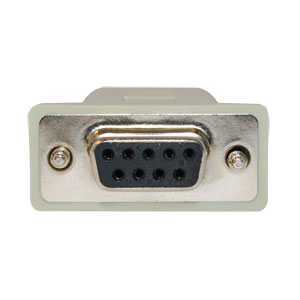
\includegraphics[width=1.5cm]{images/serial-port.jpg}}
	    \onslide<2-4>{\item PS/2接口~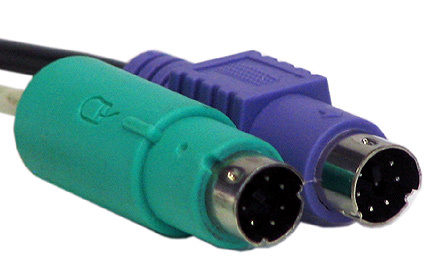
\includegraphics[width=1.5cm]{images/ps2-port.jpg}}
	    \onslide<3-5>{\item USB接口 Universal Serial Bus\\
	    	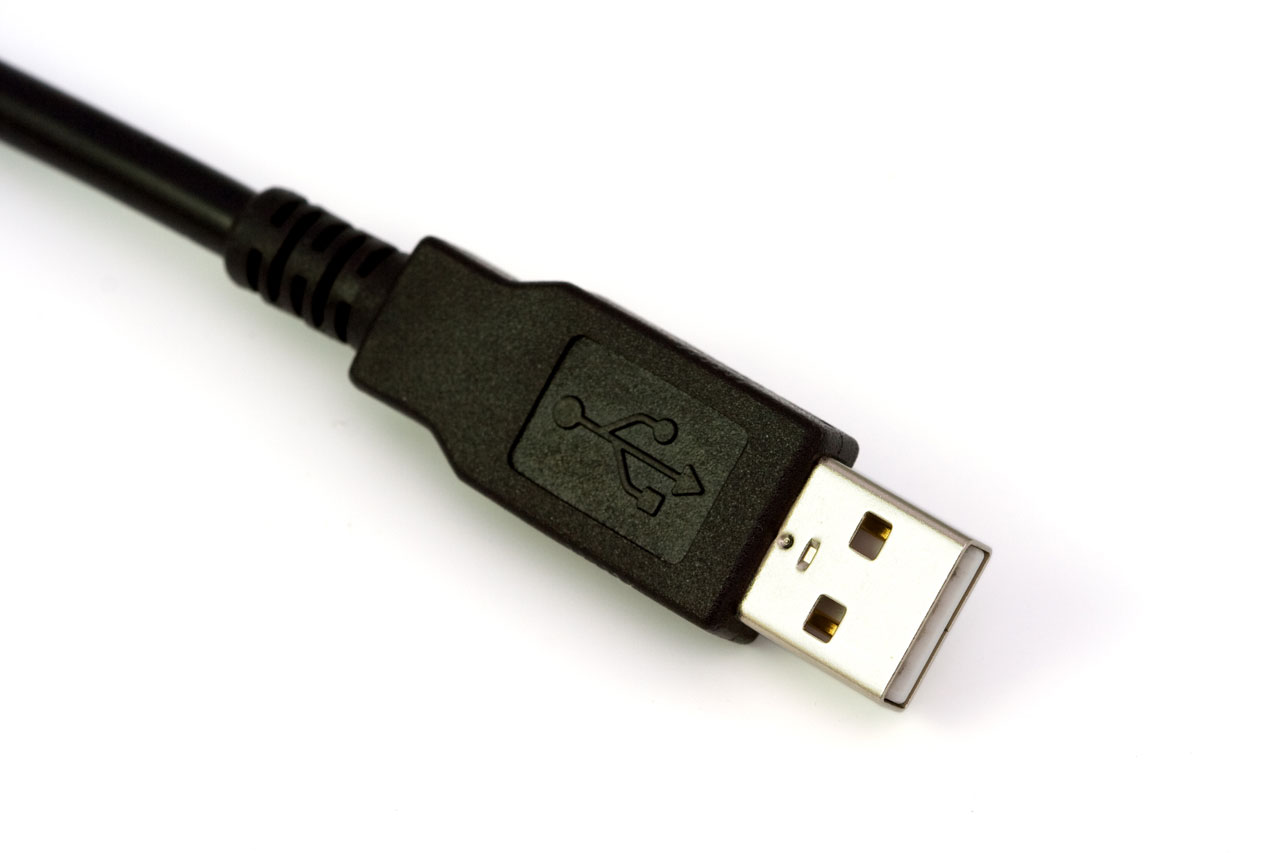
\includegraphics[width=1.5cm]{images/usb-port.jpg}~}
	    \onslide<5>{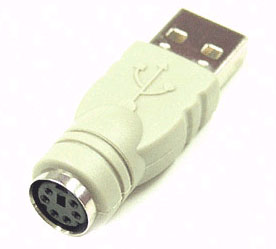
\includegraphics[width=1.5cm]{images/ps2-usb-adapter.jpg}}
	    \onslide<4-5>{\item 蓝牙接口 Bluetooth~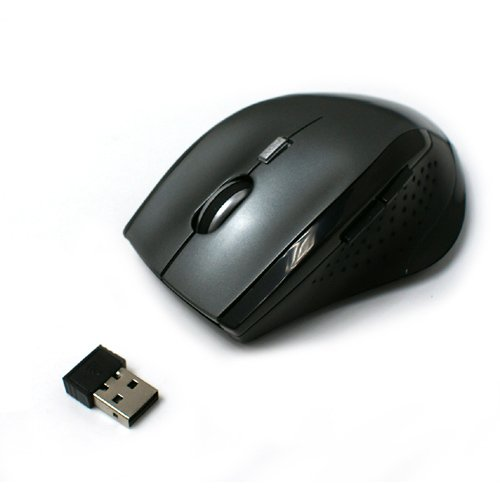
\includegraphics[width=1.5cm]{images/bluetooth-mouse.jpg}}
	\end{itemize}
\end{frame}

% http://www.freepatentsonline.com/6927759.html
% http://www.freepatentsonline.com/7119793.html
\begin{frame}
	\frametitle{鼠标的结构}
	\begin{center}
	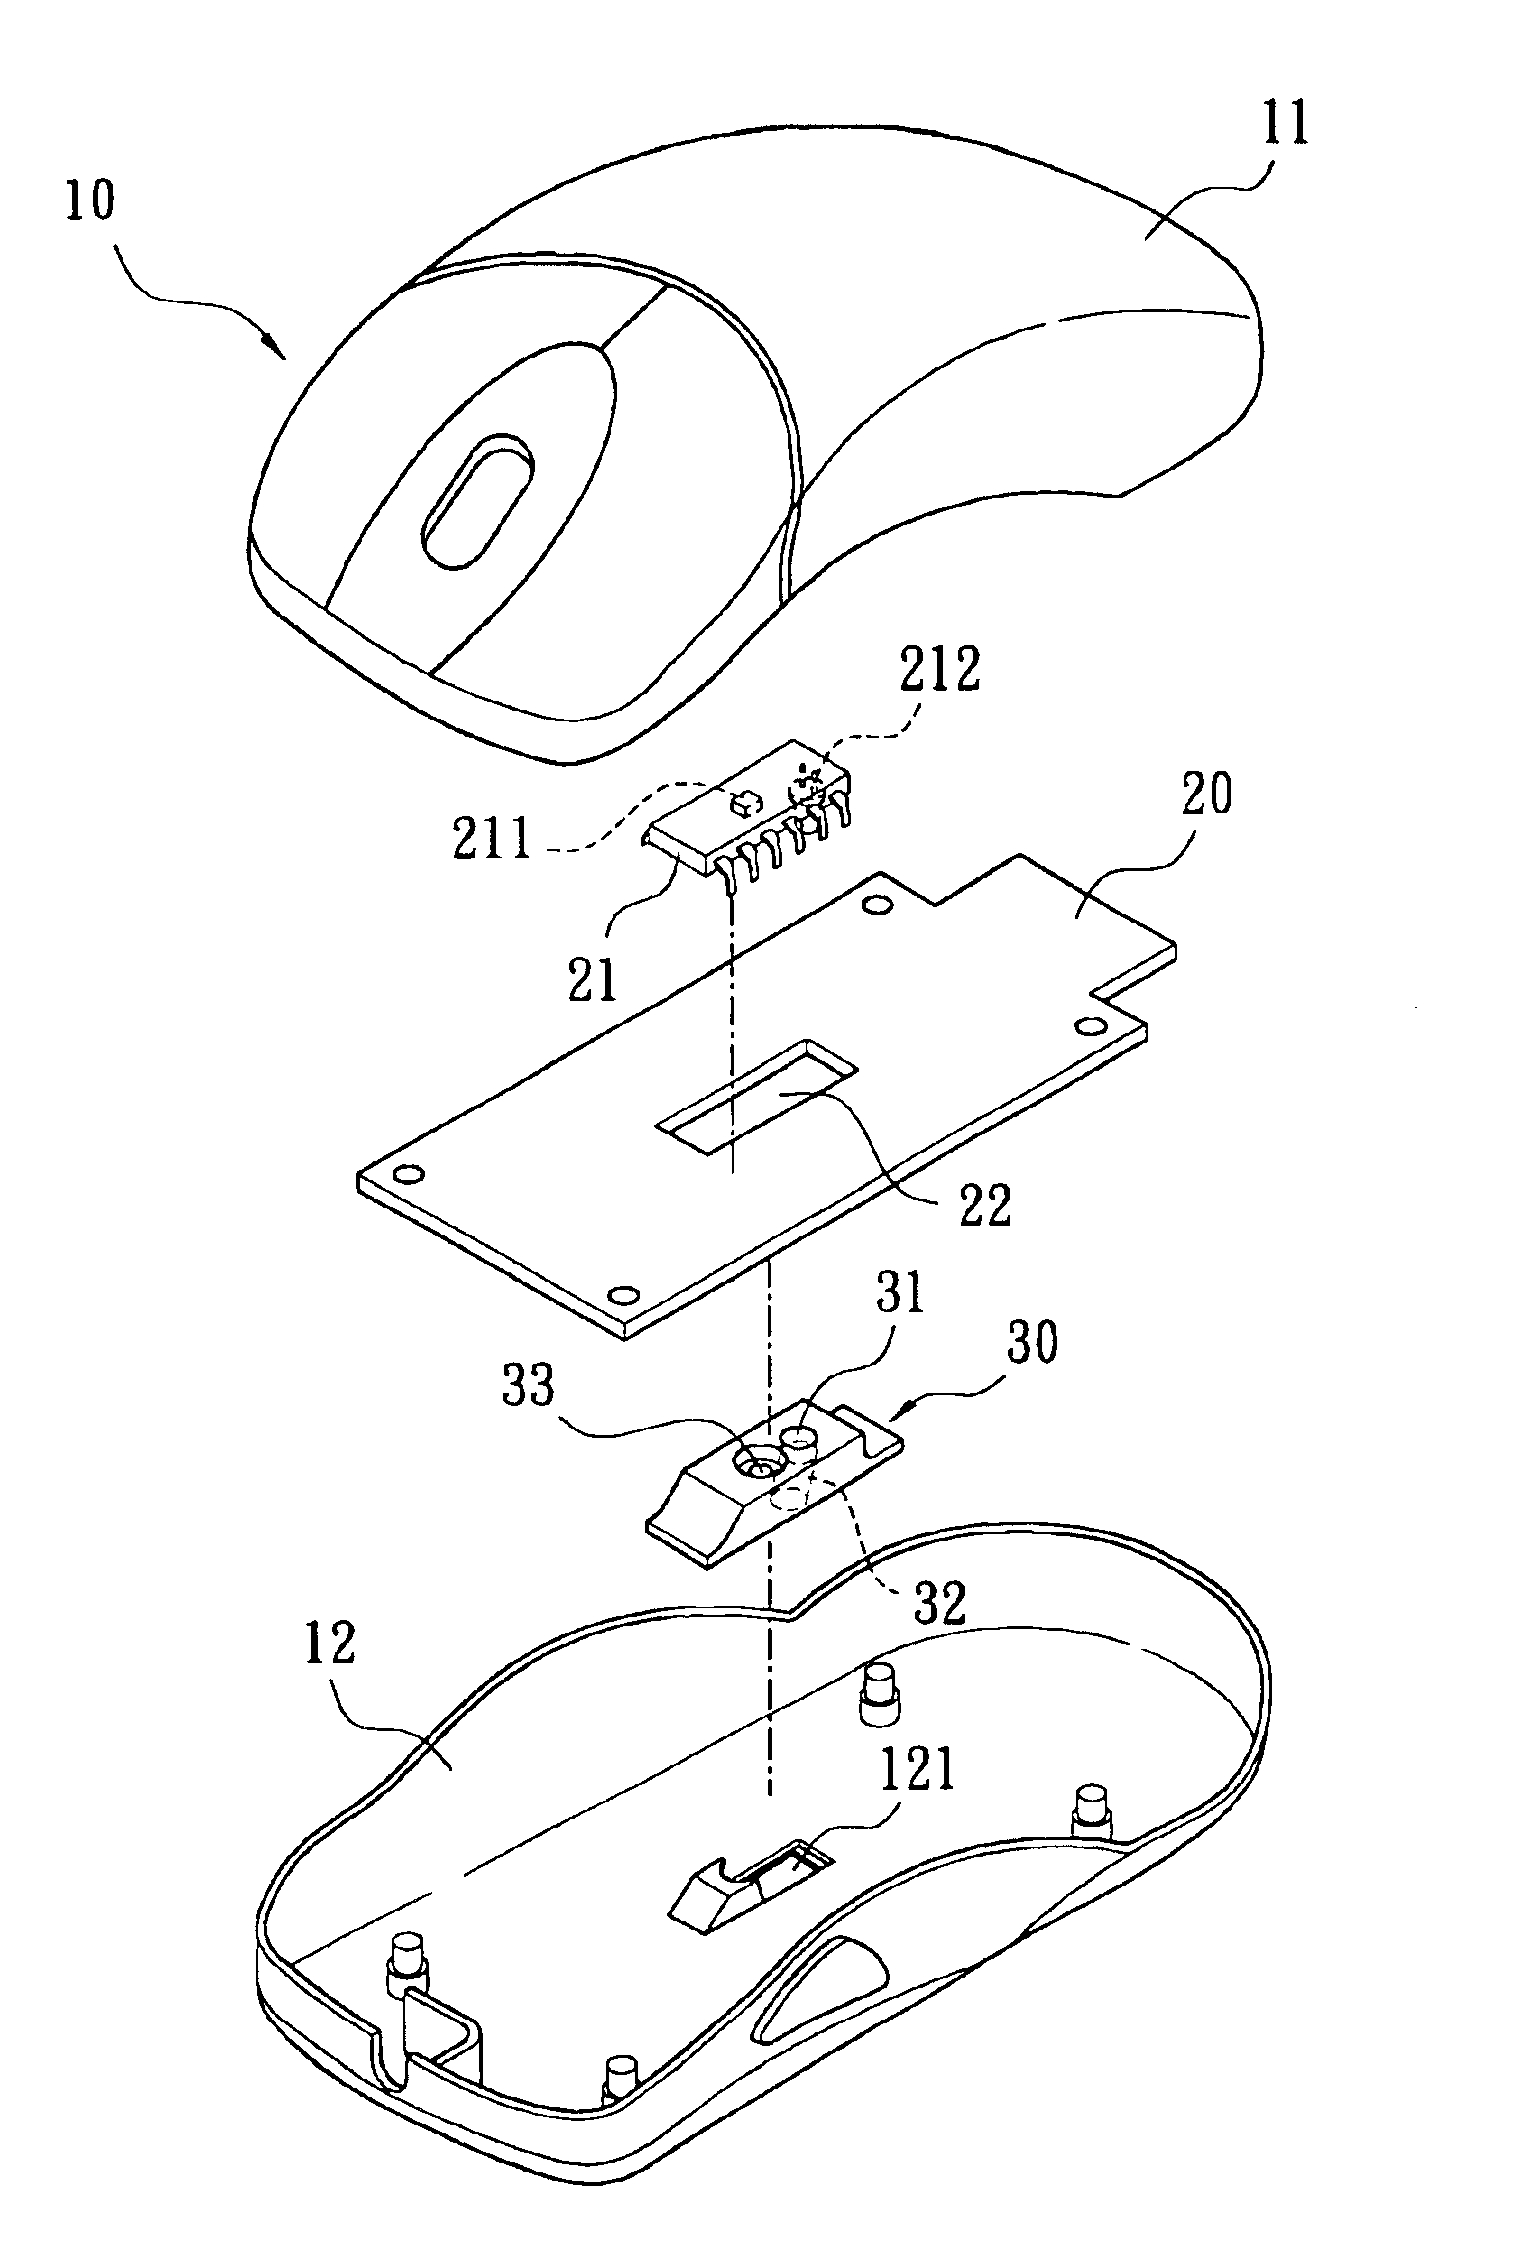
\includegraphics[scale=0.4]{images/6927759-0-large.jpg}~
	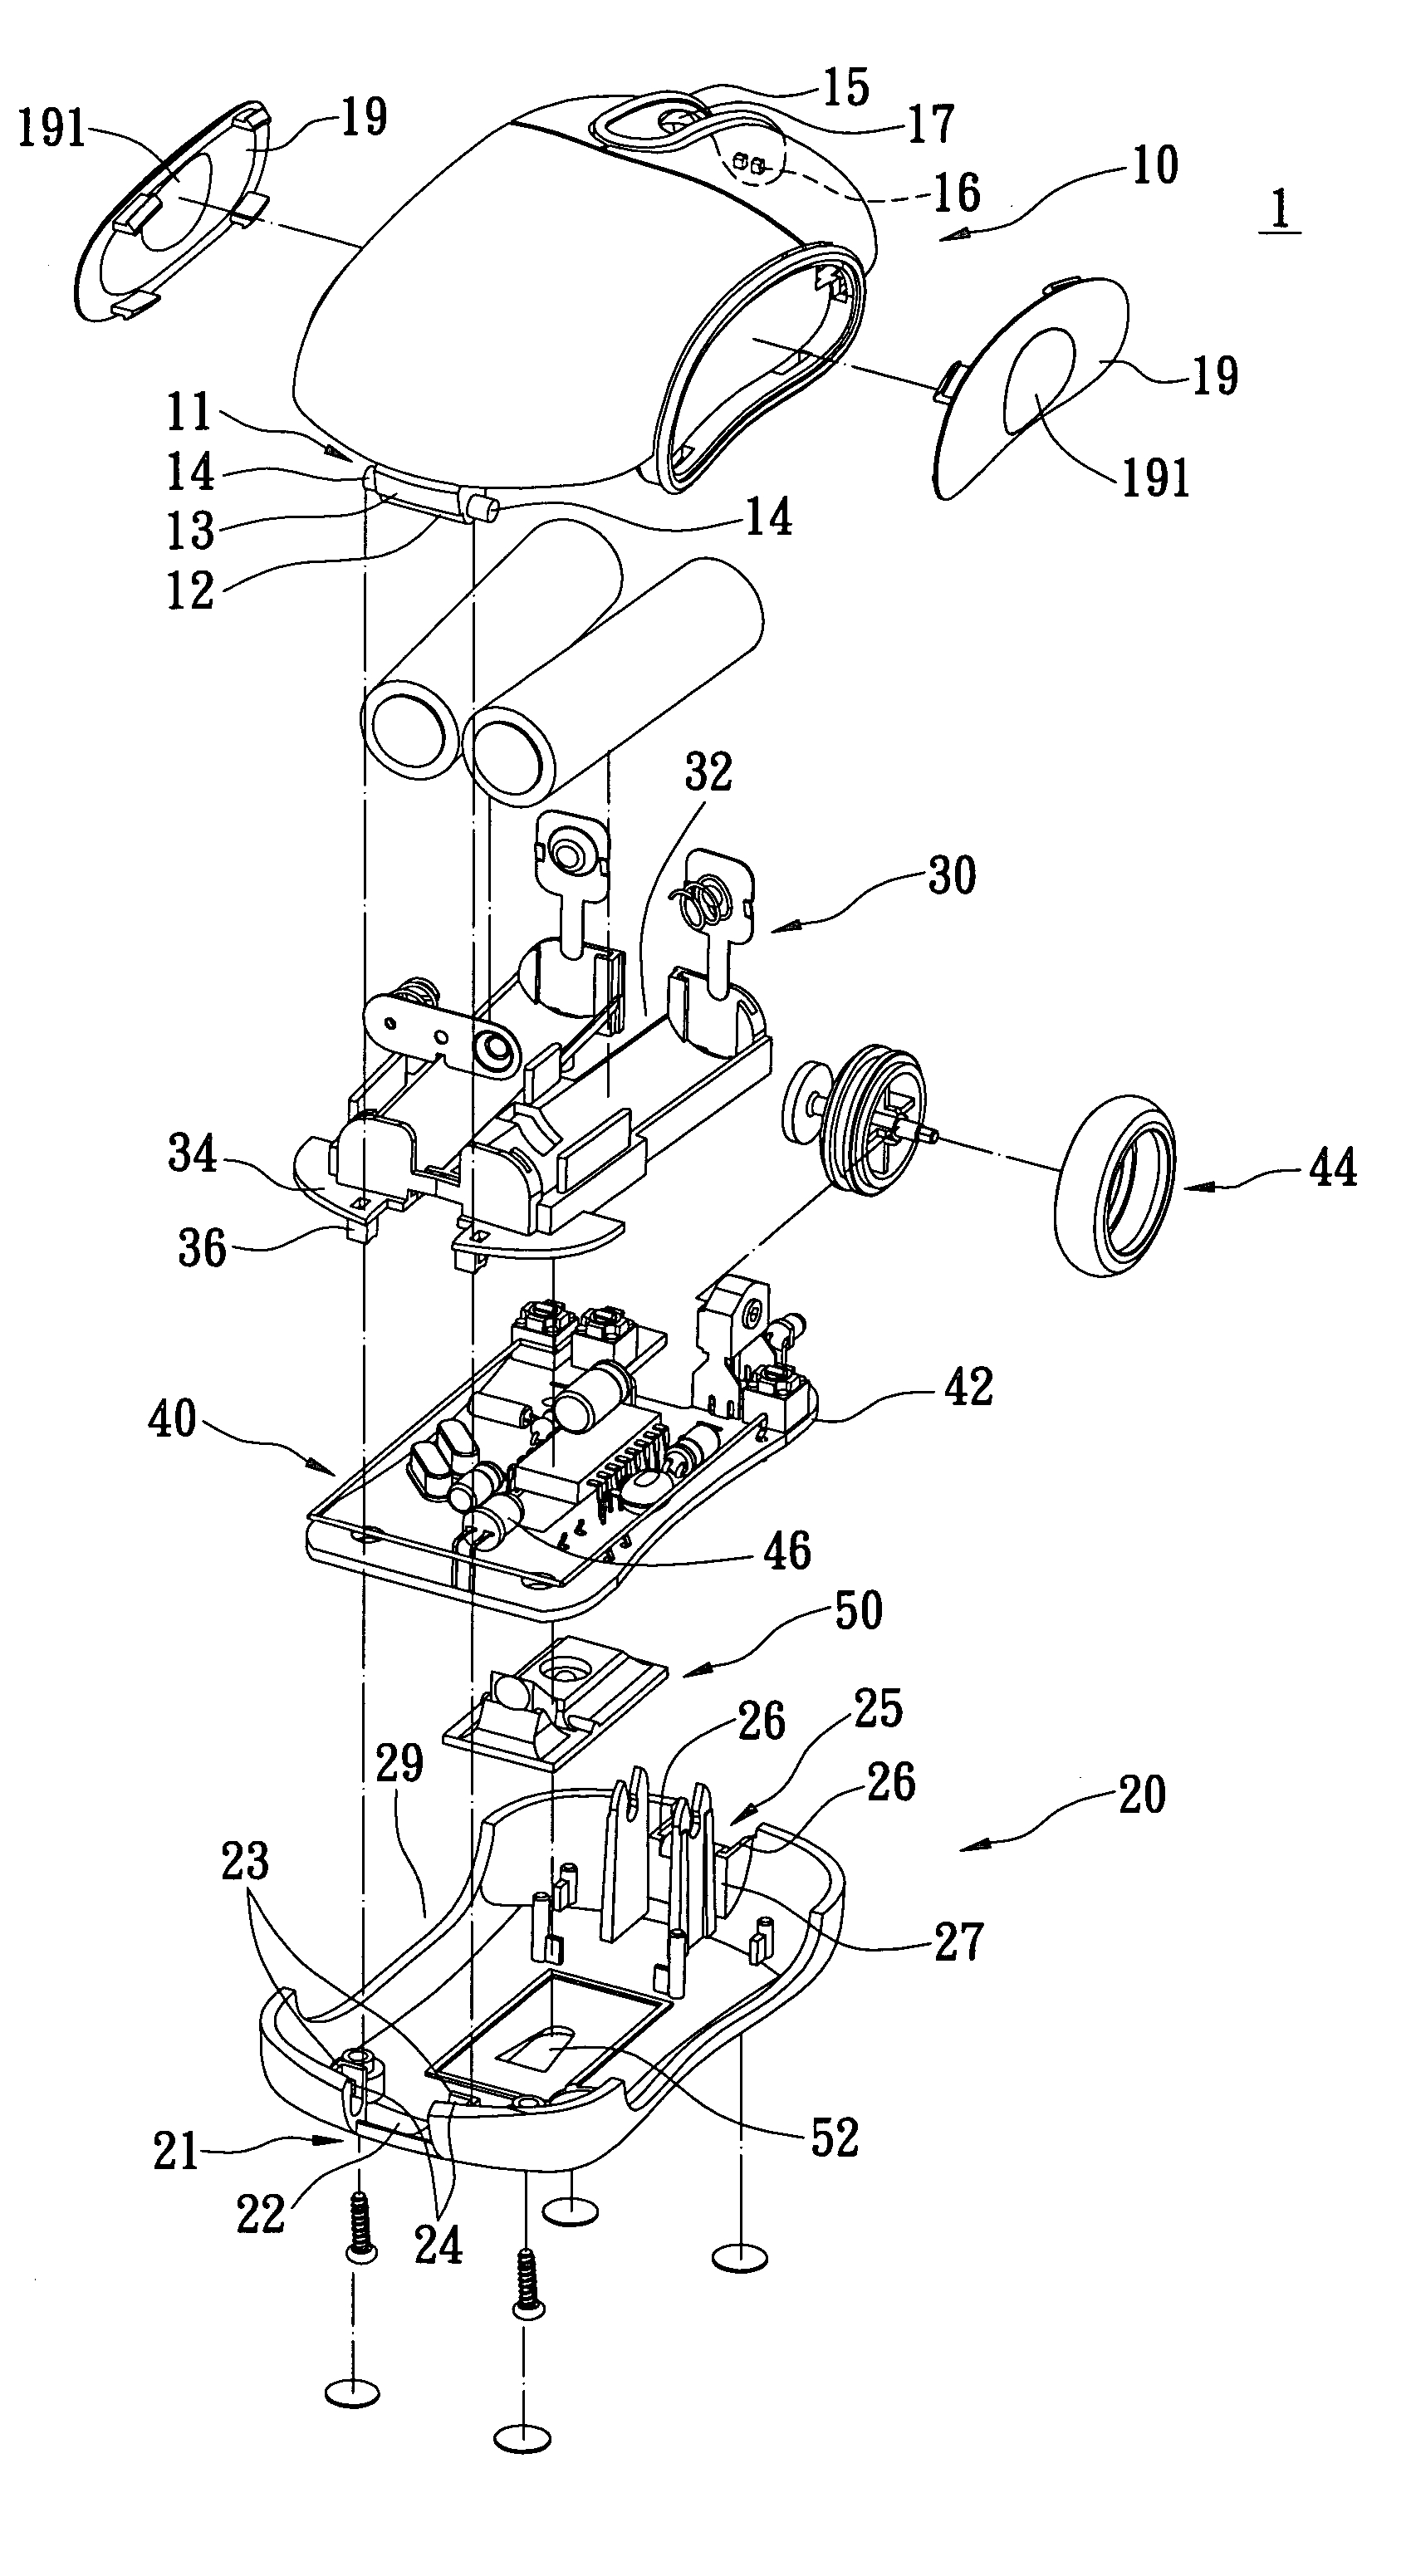
\includegraphics[scale=0.2]{images/7119793-0-large.jpg}
	\end{center}
\end{frame}

% http://www.engineersgarage.com/insight/how-optical-mouse-works
\fullPageImage{images/optical-mouse-insight-1.jpg}{\transwipe}
\fullPageImage{images/optical-mouse-insight-2.jpg}{\transwipe}
\fullPageImage{images/optical-mouse-insight-3.jpg}{\transwipe}
\fullPageImage{images/optical-mouse-insight-4.jpg}{\transwipe}
\fullPageImage{images/optical-mouse-insight-5_1.jpg}{\transwipe}
\fullPageImage{images/optical-mouse-insight-6_0.jpg}{\transwipe}
\fullPageImage{images/optical-mouse-insight-7_1.jpg}{\transwipe}
\fullPageImage{images/optical-mouse-insight-8.jpg}{\transwipe}
\fullPageImage{images/optical-mouse-insight-9.jpg}{\transwipe}
\fullPageImage{images/optical-mouse-insight-10.jpg}{\transwipe}
\fullPageImage{images/optical-mouse-insight-11.jpg}{\transwipe}
\fullPageImage{images/optical-mouse-insight-12.jpg}{\transwipe}
\fullPageImage{images/optical-mouse-insight-13.jpg}{\transwipe}

\begin{frame}
	\frametitle{鼠标的原理}
	\transdissolve
	\begin{center}
	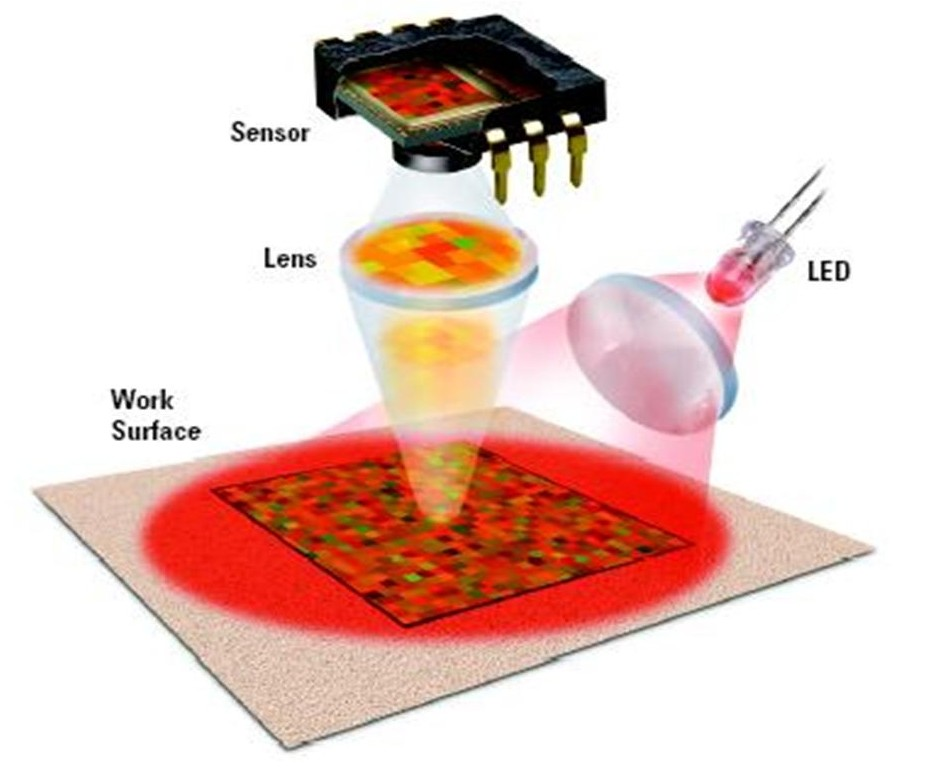
\includegraphics[width=4cm]{images/mouse-basics-1.jpg}
	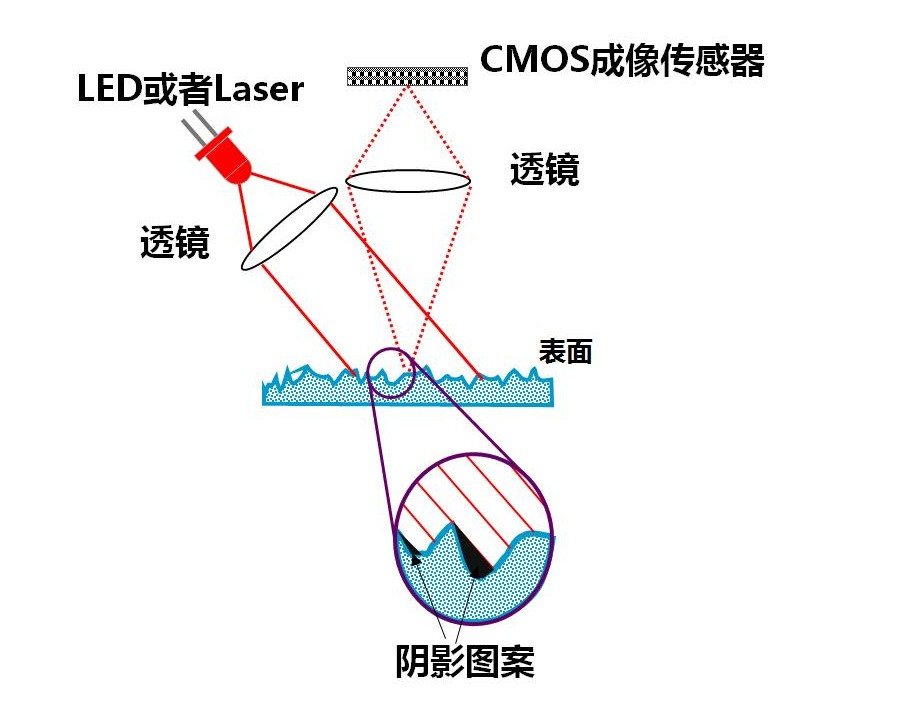
\includegraphics[width=4cm]{images/mouse-basics-2.jpg}\\
	\pause
	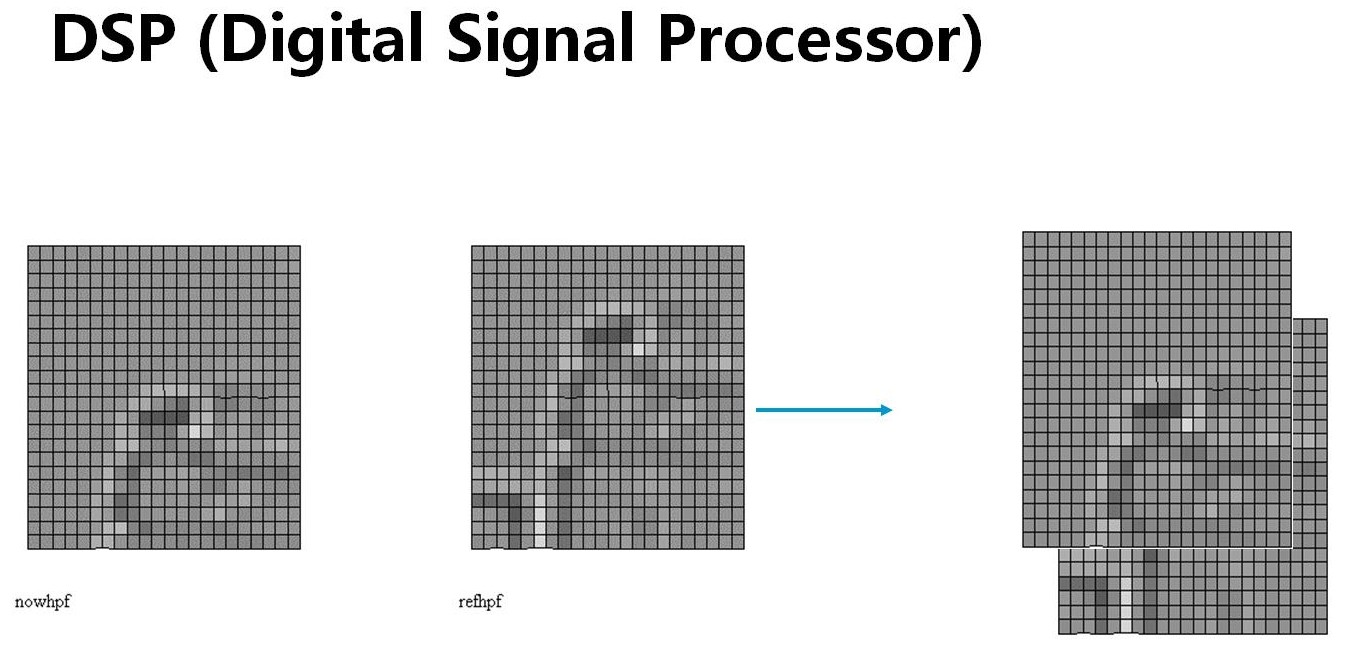
\includegraphics[width=3cm]{images/mouse-basics-3.jpg}
	\end{center}
\end{frame}

\begin{frame}
	\frametitle{新型鼠标}
	\transdissolve
	\begin{center}
	% http://www.tuvie.com/future-mouse-from-swiftpoint/
	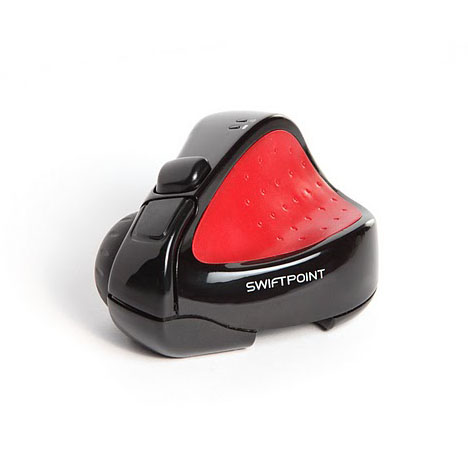
\includegraphics[width=3cm]{images/swiftpoint-mouse1.jpg}\\
	\pause
	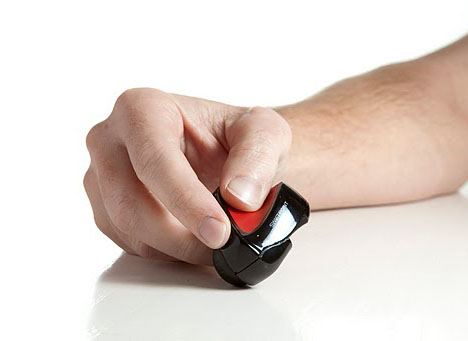
\includegraphics[width=4cm]{images/swiftpoint-mouse3.jpg}
	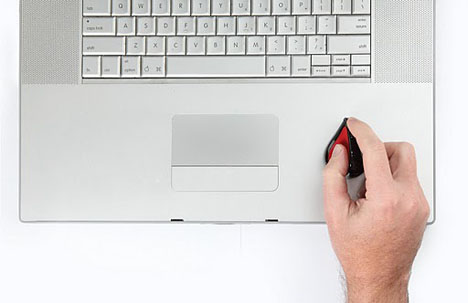
\includegraphics[width=4cm]{images/swiftpoint-mouse6.jpg}
	\end{center}
\end{frame}

% http://www.zdnet.com/wearable-tech-6-future-tech_p10-7000002331/
\fullPageImage{images/wearable-airmouse-future-computer-gadget-02-620x.jpg}{\transdissolve}

% http://archive.techtree.com/techtree/jsp/article.jsp?article_id=88590&cat_id=505
\fullPageImage{images/spacenavigator-3d-mouse2.jpg}{
	\transdissolve
	\pause
	\begin{center}
	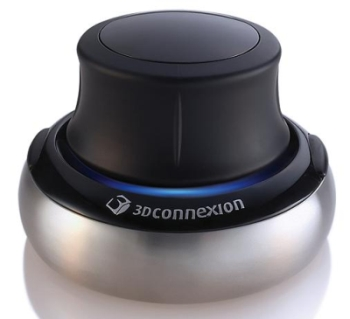
\includegraphics[width=5cm]{images/spacenavigator-3d-mouse1.jpg}
	\end{center}
}

\begin{frame}
	\frametitle{触摸板 TouchPad}
	\begin{center}
	% http://www.fayerwayer.com/up/2009/06/macbook-unibody-touchpad.jpg
	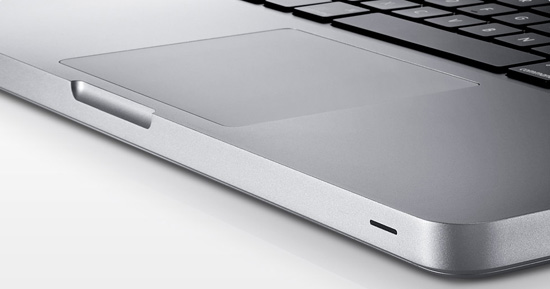
\includegraphics[width=8cm]{images/macbook-unibody-touchpad.jpg}
	\end{center}
	\begin{itemize}
		\item 移动PC的鼠标
		\begin{itemize}
			\item 由一块能够感应手指运行轨迹的压感板和两个按钮组成,电容感应
			\item 无机械磨损,控制精度不错,操作方便,易于掌握
			\item 易受污渍、水分影响
		\end{itemize}
	\end{itemize}
\end{frame}

% http://www.thinkpads.com/wp-content/gallery/lenovo-thinkpad-t410-review/
\fullPageImage{images/lenovo-thinkpad-t410-touchpad-trackpoint-ultranav.jpg}{
	\transdissolve
	\pause
	% http://www.no-ack.org/2010/12/disable-buttons-of-synaptics-touchpad.html
	\begin{center}
	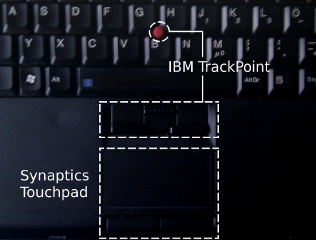
\includegraphics[width=5cm]{images/thinkpad-with-synaptics-touchpad.png}
	\end{center}
}

\begin{frame}
	\frametitle{控制杆 Joy Stick}
	% http://www.atariarchives.org/ccc/chapter5.php
	\begin{center}
	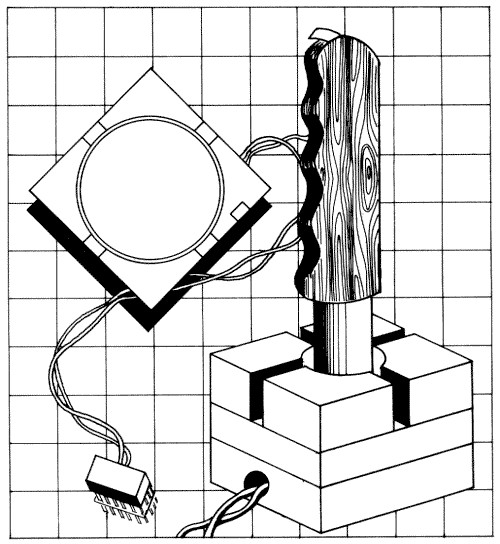
\includegraphics[height=5cm]{images/joystick-prototype-fig1.jpg}
	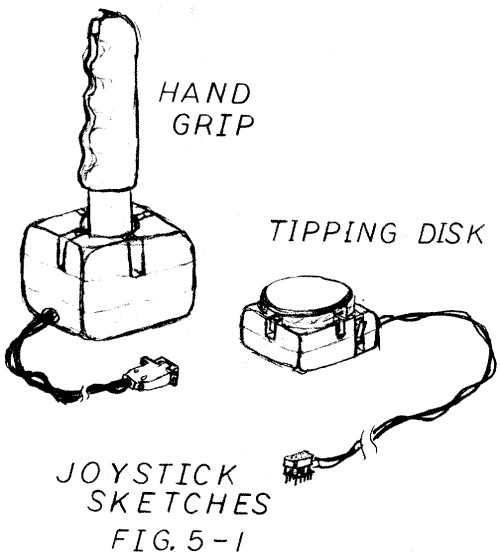
\includegraphics[height=5cm]{images/joystick-prototype-fig2.jpg}
	\end{center}
\end{frame}

\begin{frame}
	\frametitle{控制杆 Joy Stick}
	\transwipe
	\transduration<1,2,3>{.2} % Show slide specified number of seconds
	\begin{center}
	% http://radialmind.blogspot.com/2010/05/joystick-pong-how-to-write-custom-usb.html
	\includegraphics[height=2.7cm]{images/joystick1.jpg}\pause
	% http://www.hisupplier.com/product-37839-16-Bits-Joysticks/
	\includegraphics[height=2.7cm]{images/joystick2.jpg}\pause
	% http://www.technologytell.com/gaming/59500/x-arcade-solo-joystick-single-player-arcade-style-controller/
	\includegraphics[height=2.7cm]{images/x-arcade_solo_joystick_640.jpg}\pause
	\end{center}
	\begin{itemize}
		\item 将物理动作(手部的运动)转换成数字形式
		\item 早已在各种机械设备上得到应用(战斗机、挖掘机)
		\item 监视每一个轴的位置以确定操纵杆的位置
	\end{itemize}
\end{frame}

% http://baike.baidu.com/view/10658.htm
\begin{frame}
	\frametitle{触摸屏 Touch Screen}
	\beamertemplatetransparentcovereddynamicmedium
	\begin{columns}
	\column{.6\textwidth}
	\begin{itemize}[<+->]
		\item 触控是目前最简单、方便、自然的一种人机交互方式。
		\begin{itemize}
			\item 当用户接触屏幕上的图形按钮,屏幕上的触觉反馈系统可根据预先编制的程序执行各种功能。
			\item 可用以取代机械式的按钮面板,并借由液晶显示画面制造出生动的影音效果。
		\end{itemize}
	\end{itemize}
	\column{.4\textwidth}
	\includegraphics[width=4cm]{images/touch-screen.jpg}
	\end{columns}
\end{frame}

% http://www.eizo.com/global/library/basics/basic_understanding_of_touch_panel/
\begin{frame}
	\frametitle{触摸屏的应用}
	\begin{itemize}
	\item 广泛用于从ATM、售货机、导航、娱乐到手机\dots
	\end{itemize}
	\includegraphics[width=\textwidth]{images/touch-screen-applications.jpg}
\end{frame}

% http://www.planarembedded.com/technology/touch/
\begin{frame}
	\frametitle{触摸屏的组成与分类}
%	\beamertemplatetransparentcovereddynamicmedium
	\begin{columns}
	\column{.5\textwidth}
	\begin{itemize}[<+->]
		\item 矢量压力传感技术触摸屏\\
			{\tiny 早期技术}
		\item 电阻技术触摸屏\\
			{\tiny 单触,定位准确,易磨损}
		\item 电容技术触摸屏\\
			{\tiny 不易磨损、生物电、漂移}
		\item 红外线技术触摸屏\\
			{\tiny 早期:光干扰、曲面失真\\改进:免电流/压和静电干扰,适宜恶劣环境}
		\item 表面声波技术触摸屏\\
			{\tiny 在公共场所使用较多,污渍影响}
	\end{itemize}
	\column{.5\textwidth}
	\only<2>{\includegraphics[width=4.5cm]{images/resistive-how-final.jpg}}
	\only<3>{
		\includegraphics[width=3.5cm]{images/capacitive-how-final.jpg}\\
		\includegraphics[width=3.5cm]{images/projected-cap-final.jpg}
	}
	\only<4>{\includegraphics[width=4.5cm]{images/ir-how-final.jpg}}
	\only<5>{\includegraphics[width=4.5cm]{images/saw-final.jpg}}
	\end{columns}
\end{frame}

% http://www.ecnmag.com/articles/2010/04/advances-touch-controller-technology
\fullPageImage{images/pct-construction.jpg}{\transdissolve}

% http://electronicdesign.com/article/components/self-capacitive-sensing-brings-touch-to-large-screens-
% http://www.radio-electronics.com/articles/electronics-components/touchscreen-controller---key-points-to-25
% http://bbs.ednchina.com/BLOG_ARTICLE_38488.HTM (中文版)
\fullPageImage{images/pct-construction-comparision.png}{\transwipe}

% http://medialoot.com/item/40-vector-multitouch-gestures/
\begin{frame}
	\frametitle{多点触摸}
	\includegraphics[width=\textwidth]{images/640x440_Vector_MultiTouch_Gestures_Preview3.png} 
\end{frame}

% http://www.gizmowatch.com/entry/perceptive-pixel-uncovers-gigantic-82-inch-pro-cap-lcd-display/
\fullPageImage{images/biggest_projected_capacitive_display_r7p8n.jpg}{\transdissolve}
% http://www.knowledgebase-script.com/demo/article-420.html
\fullPageImage{images/microsoft-surface.jpg}{\transwipe}
\fullPageImage{images/microsoft-surface-illustration.jpg}{
	\transwipe
	\begin{beamerboxesrounded}[shadow=true]{关键环节}
		\only<1>{1. 屏幕:多用户同时进行多点触控输入}
		\only<2>{2. 红外:在近红外波长范围探测搁置物}
		\only<3>{3. 处理器:Core 2 Duo处理器, 2GB内存256MB显存,蓝牙、Wifi \dots}
		\only<4>{4. 投影:1024 x 768分辨率高清投影}
	\end{beamerboxesrounded}
}
%1. Screen: A diffuser turns the Surface's acrylic tabletop into a large horizontal "multitouch" screen, capable of processing multiple inputs from multiple users. The Surface can also recognize objects by their shapes or by reading coded "domino" tags.
%2. Infrared: Surface's "machine vision" operates in the near-infrared spectrum, using an 850-nanometer-wavelength LED light source aimed at the screen. When objects touch the tabletop, the light reflects back and is picked up by multiple infrared cameras with a net resolution of 1280 x 960.
%3. CPU: Surface uses many of the same components found in everyday desktop computers. A Core 2 Duo processor, 2GB of RAM and a 256MB graphics card. Wireless communication with devices on the surface is handled using WiFi and Bluetooth antennas (future versions may incorporate RFID or Near Field Communications). The underlying operating system is a modified version of Microsoft Vista.
%4. Projector: Microsoft's Surface uses the same DLP light engine found in many rear-projection HDTVs. The footprint of the visible light screen, at 1024 x 768 pixels, is actually smaller than the invisible overlapping infrared projection to allow for better recognition at the edges of the screen.

\subsubsection{图像输入设备}
\begin{frame}
	\frametitle{图像输入设备}
	\begin{itemize}
		\item 图像输入是人与计算机交互的另外一个重要组成部分。
		\begin{itemize}
			\item 静态画面\\{\tiny \textbf{数码相机、二维扫描仪},快速输入图像,且经过对图像的分析与识别,可以得到文字、图形等内容;}
			\item 动态画面\\{\tiny \textbf{摄像头},捕捉动态场景。}
		\end{itemize}
	\end{itemize}
	\begin{center}
	\includegraphics[width=.25\textwidth]{images/scanner.jpg}
	\includegraphics[width=.25\textwidth]{images/scanner-barcode.jpg}
	\includegraphics[width=.25\textwidth]{images/camera.jpg}
	\includegraphics[width=.25\textwidth]{images/compact_camera.jpg}
	\end{center}
\end{frame}

\begin{frame}
	\frametitle{扫描仪}
	\beamertemplatetransparentcovereddynamicmedium
	\begin{columns}
	\column{.6\textwidth}
	\begin{enumerate}[<+->]
		\item {\small 光源将光线照射到待扫描的图像原稿上,产生反射光或透射光;}
		\item {\small 经反光镜组反射到电荷耦合器件 (Charge Coupled Device, CCD)中;}
		\item {\small CCD图像传感器根据反射光线强弱的不同转换成不同大小的电流;}
		\item {\small 电流经模拟/数字转换处理,将电信号转换成数字信号,即产生一行图像数据。}
	\end{enumerate}
	\column{.4\textwidth}
	% (obsolete) http://www.pcmag.com/article2/0,2817,1156000,00.asp
	% http://www.petervaldivia.com/eso/computers/computers.php
	\includegraphics[width=.9\textwidth]{images/scanner-diagram.jpg}
	\end{columns}
\end{frame}

\begin{frame}
	\frametitle{扫描仪~{\small 分辨率}}
	\beamertemplatetransparentcovereddynamicmedium
	\begin{itemize}[<+->]
		\item 分辨率决定了最高扫描精度\\{\tiny 高分辨率意味着高图像精度,还将增加扫描文件尺寸。}
		\item 光学分辨率\\{\tiny 光学部件 (即透镜组) 分辨率 + 传感器 (即CCD器件) 分辨率}
		\item 插值分辨率\\{\tiny 由驱动程序及后期处理软件进行处理,如拟合、锐化\dots ,将增加图像像素。}
	\end{itemize}
\end{frame}

\begin{frame}
	\frametitle{扫描仪~{\small 扫描速度}}
	\beamertemplatetransparentcovereddynamicmedium
	\begin{itemize}[<+->]
		\item 一般指扫描仪从预览开始到图像扫描完成后,光头移动的时间,即物理部件工作过程用时。
		\item 有时把扫描图像送到word文档中所花费的时间,往往比单纯的扫描过程还要长。
		\item 完整的扫描速度:
		\begin{itemize}
			\item 作业任务从打开扫描仪完成预热,到把从原稿放置在扫描平台上开始,到最终完成图像处理的整个过程。
		\end{itemize}
	\end{itemize}
\end{frame}

% http://h20424.www2.hp.com/product/scanjet/cn/zh/index.asp
\begin{frame}
	\frametitle{扫描仪~{\small 扫描速度}}
	\begin{columns}
		\column{.5\textwidth}
		\begin{itemize}
			\item {\small HP Scanjet Enterprise 7000n 文档捕获工作站}
			\item {\tiny 600 dpi分辨率,48位色彩深度}
			\item {\tiny 扫描速度(ADF、A4): }
			\begin{itemize}
				\item {\tiny \textbf{40 页/分钟/80 幅图像/分钟(黑白和灰阶)}}
				\item {\tiny \textbf{35 页/分钟/70 幅图像/分钟(彩色)}}
			\end{itemize}
			\item {\tiny 最大扫描尺寸(平板): 216 x356 毫米}
			\item {\tiny 支持的介质类型: }
			\begin{itemize}
				\item {\tiny 普通纸、喷墨纸;信封、标签、卡片}
			\end{itemize}
			\item {\tiny 日打印负荷 2000 页}
		\end{itemize}
		\column{.5\textwidth}
		\includegraphics[width=.9\textwidth]{images/scanjet7000.jpg}
	\end{columns}
\end{frame}

% http://www.photoreview.com.au/news/canon-unveils-long-awaited-eos-5d-mark-ii
\fullPageImage{images/canon-5d2-front-view_sml.jpg}{\transwipe}
\fullPageImage{images/canon-5d2-k218frontview_sml.jpg}{\transwipe}

% http://images04.olx.co.id/ui/11/90/25/1346258522_433538525_1-Gambar--Nokia-808-PureView-Harga-Rp3700000-Call-62856-5639-7135.jpg
\fullPageImage{images/Nokia-808-PureView-Harga.jpg}{\transwipe}
% Kamera utama 41 MP (38 MP effective, 7152 x 5368 pixels), Carl Zeiss optics, autofocus, Xenon flash, 1/1.2 sensor size, ND filter, up to 3x loseless digital zoom, geo-tagging, face detection, Video 1080p@30fps

% http://www.esato.com/news/under-the-cover-of-nokia-808-pureview-2333#g221
\fullPageImage{images/inside-the-nokia-808-pureview-lens.jpg}{\transwipe}
% http://conversations.nokia.com/2012/03/01/nokia-pureview-qa-with-damian-dinning/
\fullPageImage{images/pureview-detached.jpg}{\transwipe}
%http://www.engadget.com/2012/03/05/nokia-808-shows-off-carl-zeiss-lens-division/
\fullPageImage{images/pureview-lens.jpg}{\transwipe}
% http://media.gizmodo.co.uk/wp-content/uploads/2012/09/original.jpg
\fullPageImage{images/pureview-comparision.jpg}{\transwipe}

% http://http://www.appvv.com/news/2670.shtml
% 苹果的这个专利被命名为“配备不同照相机镜头的便携式电子设备背板”(Back Panel for a Portable Electronic Device with Different Camera Lens Options)。专利文件显示,随着用高压缩设备拍出的数码图片的质量越来越高,用户希望能获得在高端数码相机(如数码单反相机)上拥有的一些更复杂的功能,这需要为设备搭配强大的镜头、滤镜、光学变焦和图像稳定器材。
\fullPageImage{images/apple-patent-camera.jpg}{\transwipe}
% http://reviews.in.88db.com/index.php/technology/digital-cameras/17146-iphone-to-get-slr-like-changeable-lenses
\fullPageImage{images/Apple-Changeable-Lens.jpg}{\transwipe}

\begin{frame}
	\frametitle{数码摄像头}
	\begin{center}
	% http://www.sciencedirect.com/science/article/pii/S1076567010620058
	\includegraphics[width=.8\textwidth]{images/ccd.jpg}
	\end{center}
\end{frame}

% http://www.tedpella.com/cameras_html/ccd_cmos.htm
\fullPageImage{images/ccd-internal.jpg}{\transwipe}
\fullPageImage{images/cmos-internal.jpg}{\transwipe}

% http://pluggedin.kodak.com/pluggedin/post/?id=2179980
\fullPageImage{images/wafer.jpg}{
	\transdissolve
	% http://www.steves-digicams.com/news/fujifilm-announces-digital-imaging-breakthrough-with-its-new-super-ccd.html
	\pause
	\begin{center}
	\includegraphics[scale=.5]{images/ccd-chip.jpg}
	\end{center}
}

\subsection{输出设备}
\begin{frame}
	\frametitle{输出设备}
	\beamertemplatetransparentcovereddynamicmedium
	\tikzstyle{punkt} = [
		rectangle,
		rounded corners,
		draw=black, very thick,
		text width=6.5em,
		minimum height=2em,
		text centered]
	\tikzstyle{line} = [
		draw,
		text centered]
	\begin{tikzpicture}[node distance=0.5cm, auto,]
		\node[punkt] (display) {显示};
		\uncover<2->{\node[punkt, right=of display] (epaper) {电子纸};}
		\node[punkt, right=of epaper] (print) {打印};
		\uncover<2->{\path[line]	(display)--(epaper);
		\path[line]	(epaper)--(print);}
	\end{tikzpicture}
\end{frame}

\subsubsection{显示器}
\begin{frame}
	\frametitle{显示器}

\end{frame}

\subsubsection{打印机}
\begin{frame}
	\frametitle{打印机}

\end{frame}

\subsubsection{电子纸与电子墨水}
% http://news.cnet.com/8301-17938_105-20009738-1/kindle-vs-nook-vs-ipad-which-e-book-reader-should-you-buy/
\fullPageImage{images/ebooks.jpg}{\transwipe}
\fullPageImage{images/kindle-inside.jpg}{\transwipe}

% http://www.economist.com/node/442911
\begin{frame}
	\frametitle{电子纸与电子墨水 Electronic Paper, Ink}
	\transwipe
	\begin{center}
	\includegraphics[height=.8\textheight, width=.6\textwidth]{images/e-ink-technology.jpg}
	\end{center}
\end{frame}

% http://www.seikowatches.com/baselworld/2007/press/details/070412_11.html
\begin{frame}
	\frametitle{电子纸与电子墨水 Electronic Paper, Ink}
	\transwipe
	\begin{center}
	\includegraphics[width=\textwidth]{images/e-ink-technology-detail.jpg}
	\end{center}
\end{frame}

% http://zh.wikipedia.org/wiki/电子纸
\begin{frame}[transwipe]
	\frametitle{电子纸与电子墨水 Electronic Paper, Ink}
	\beamertemplatetransparentcovereddynamicmedium
	\begin{itemize}[<+->]
		\item 仿效墨水在真实纸张上的显现,如同普通纸一样可以反射环境光。
		\item \textbf{不加电}的情况下可保留原先显示的图片和文字状态。
		\item 显示内容时图像固定、无需持续刷新,所显示的图像具有\textbf{很大的可视角度}。
		\item 与纸的特性十分相似,其色彩对比高、分辨率高、耗电量小、制造成本低。
		\item 应用于零售商店价签,数字标牌,电子公告牌,手机屏幕,电子书阅读器。
	\end{itemize}
\end{frame}

% http://www.seikowatches.com/baselworld/2007/press/details/070412_11.html
\begin{frame}
	\frametitle{电子纸与电子墨水 Electronic Paper, Ink}
	\transwipe
	\begin{center}
	\includegraphics[height=.8\textheight, width=.4\textwidth]{images/e-ink-watch1.jpg}
	\includegraphics[height=.8\textheight, width=.4\textwidth]{images/e-ink-watch2.jpg}
	\end{center}
\end{frame}

% http://zh.wikipedia.org/wiki/电子纸
\begin{frame}
	\frametitle{电子纸与电子墨水 Electronic Paper, Ink}
	\beamertemplatetransparentcovereddynamicmedium
	\begin{itemize}
		\item 刷新速度极低、复杂交互不便\pause
		\begin{itemize}
			\item 强制刷新清楚图像残留,搭配键盘、触屏
		\end{itemize}\pause
		\item 与液晶屏幕相比,最大的缺点是没有背光\pause
		\begin{itemize}
			\item 给电子纸搭配一个辅助光源
		\end{itemize}\pause
		\item E-Ink屏幕开始大规模上市的时候,还有两大缺陷需要改进\pause
		\begin{itemize}
			\item 一是无法进行彩色显示
			\item 二是采用玻璃基板导致重量较大而且易摔坏。
		\end{itemize}
		\item 同时将两个缺陷解决的彩色柔性电子纸技术直到最近才成熟。
	\end{itemize}
\end{frame}

% http://www.cnbeta.com/articles/206296.htm
\fullPageImage{images/glow-light.jpg}{\transwipe}
\fullPageImage{images/paper-white.jpg}{\transwipe}
\fullPageImage{images/paper-white-inside.jpg}{\transwipe}

\begin{frame}
	\frametitle{电子纸与电子墨水 Electronic Paper, Ink}
	\begin{itemize}
		\item E-Ink屏幕开始大规模上市的时候,还有两大缺陷需要改进
		\begin{itemize}
			\item 一是无法进行彩色显示
			\item 二是采用玻璃基板导致重量较大而且易摔坏。
		\end{itemize}
		\item 同时将两个缺陷解决的彩色柔性电子纸技术直到最近才成熟。
	\end{itemize}
\end{frame}

\fullPageImage{images/plastic-logic.jpg}{\transwipe}

\subsubsection{语音交互设备}
\begin{frame}
	\frametitle{语音交互设备}

\end{frame}

\section{小结}
\begin{frame}
	\frametitle{小结}
	\begin{itemize}
		\item 输入设备:
		\begin{itemize}
			\item 文本输入设备
			\item 图像输入设备
			\item 指点输入设备\dots
		\end{itemize}
		\item 输出设备:
		\begin{itemize}
			\item 显示器 
			\item 打印机
			\item 声音的输出\dots
		\end{itemize}
	\end{itemize}
\end{frame}
 
\begin{frame}
	\frametitle{参考文献}
	\bibliographystyle{plain}
	\bibliography{hci}
\end{frame}

\end{document}